\chapter{Use case}

%begin free user section
\section{Unidentified user}
	\subsection{Overview}
		\begin{figure}[ht]
			\begin{center}
				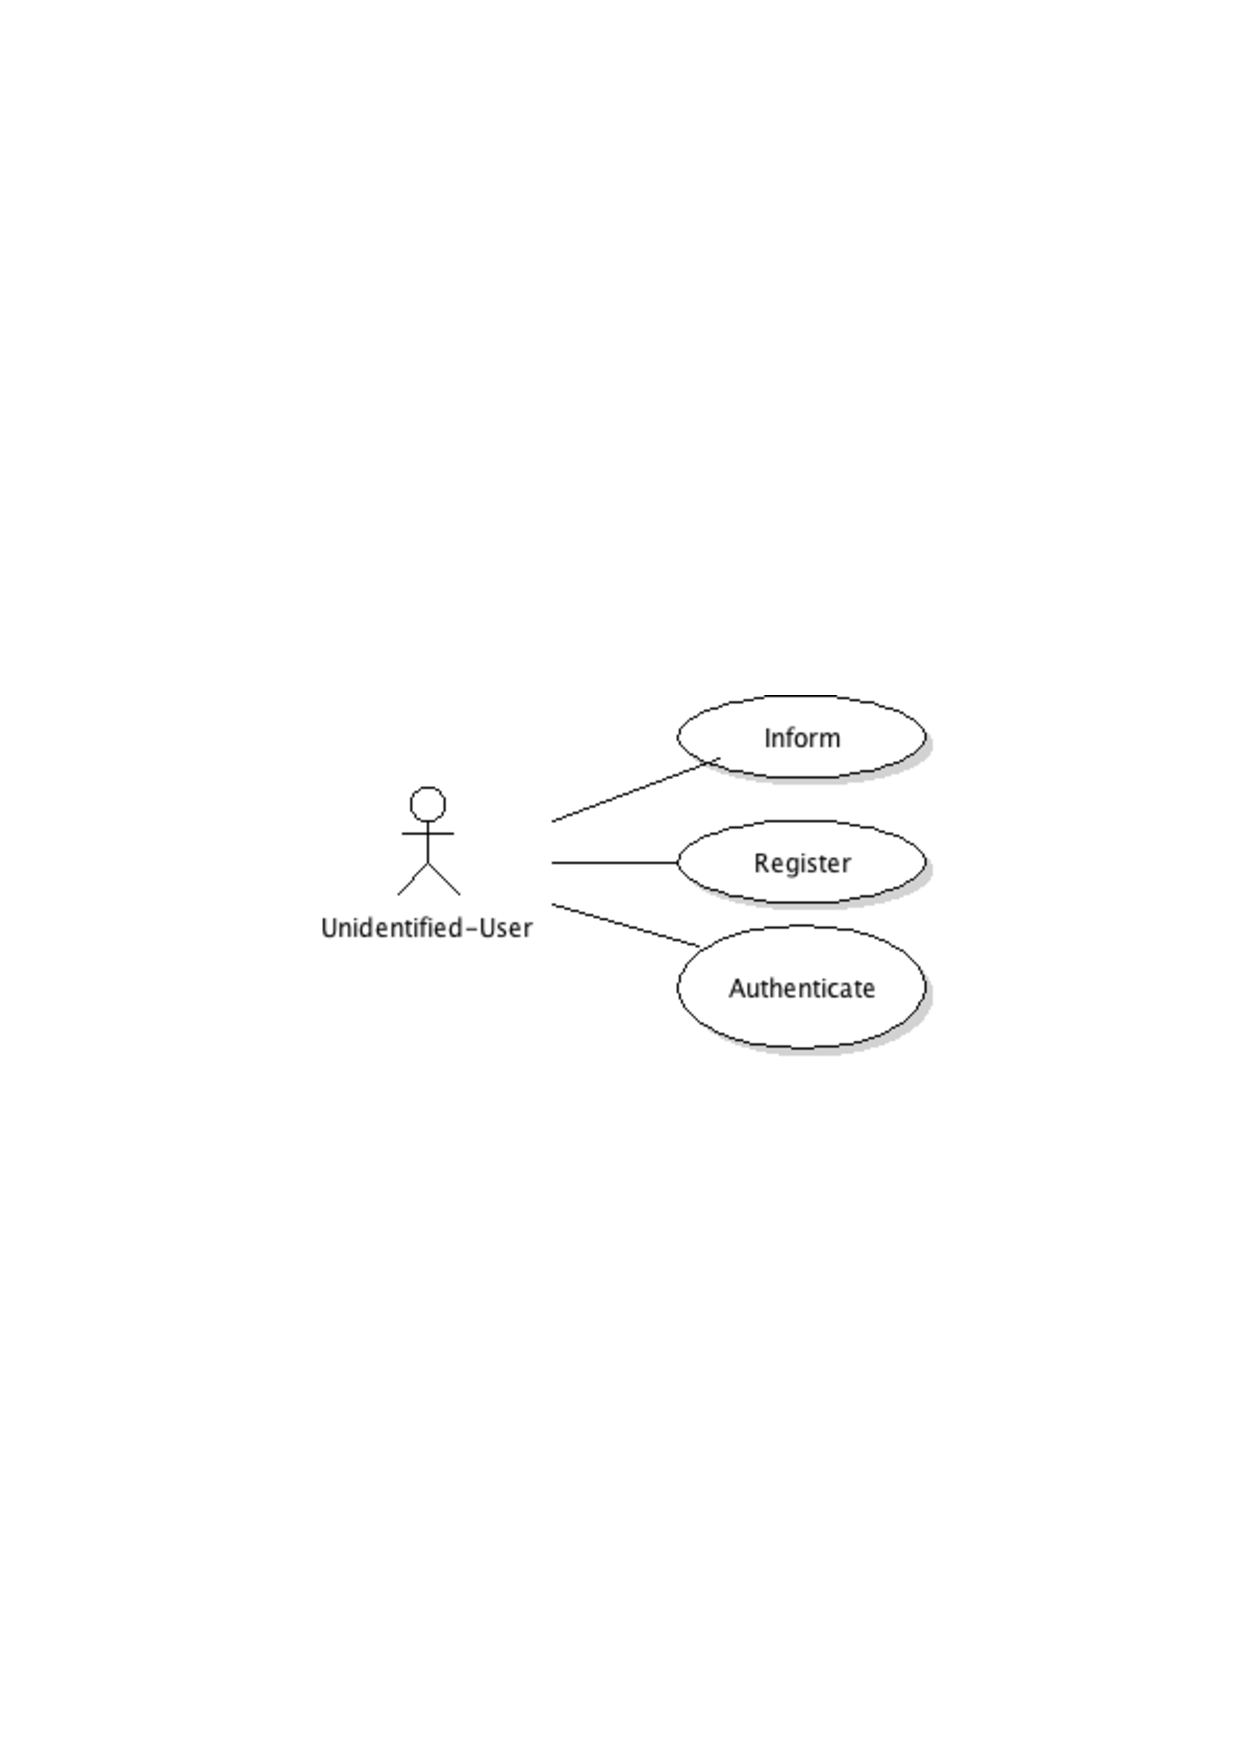
\includegraphics[width=\textwidth,  trim=2cm 12cm 2cm 11cm]{UML_figure/UC/uni_user/UC_UniUser_General.pdf}
				\caption{Unidentified user Use Case : Overview}
			\end{center}
		\end{figure}
	\subsection{Get informed}An unidentified user gets inform about the platform.
	\subsection{Register}An unidentified user who wants to access to the features of the platform has to register first.
	\subsection{Authenticate}An unidentified user authenticates to have access to the features is already registered.
%end free user section
\newpage
%begin student section
\section{Student}
	\subsection{Overview}
		\begin{figure}[ht]
			\begin{center}
				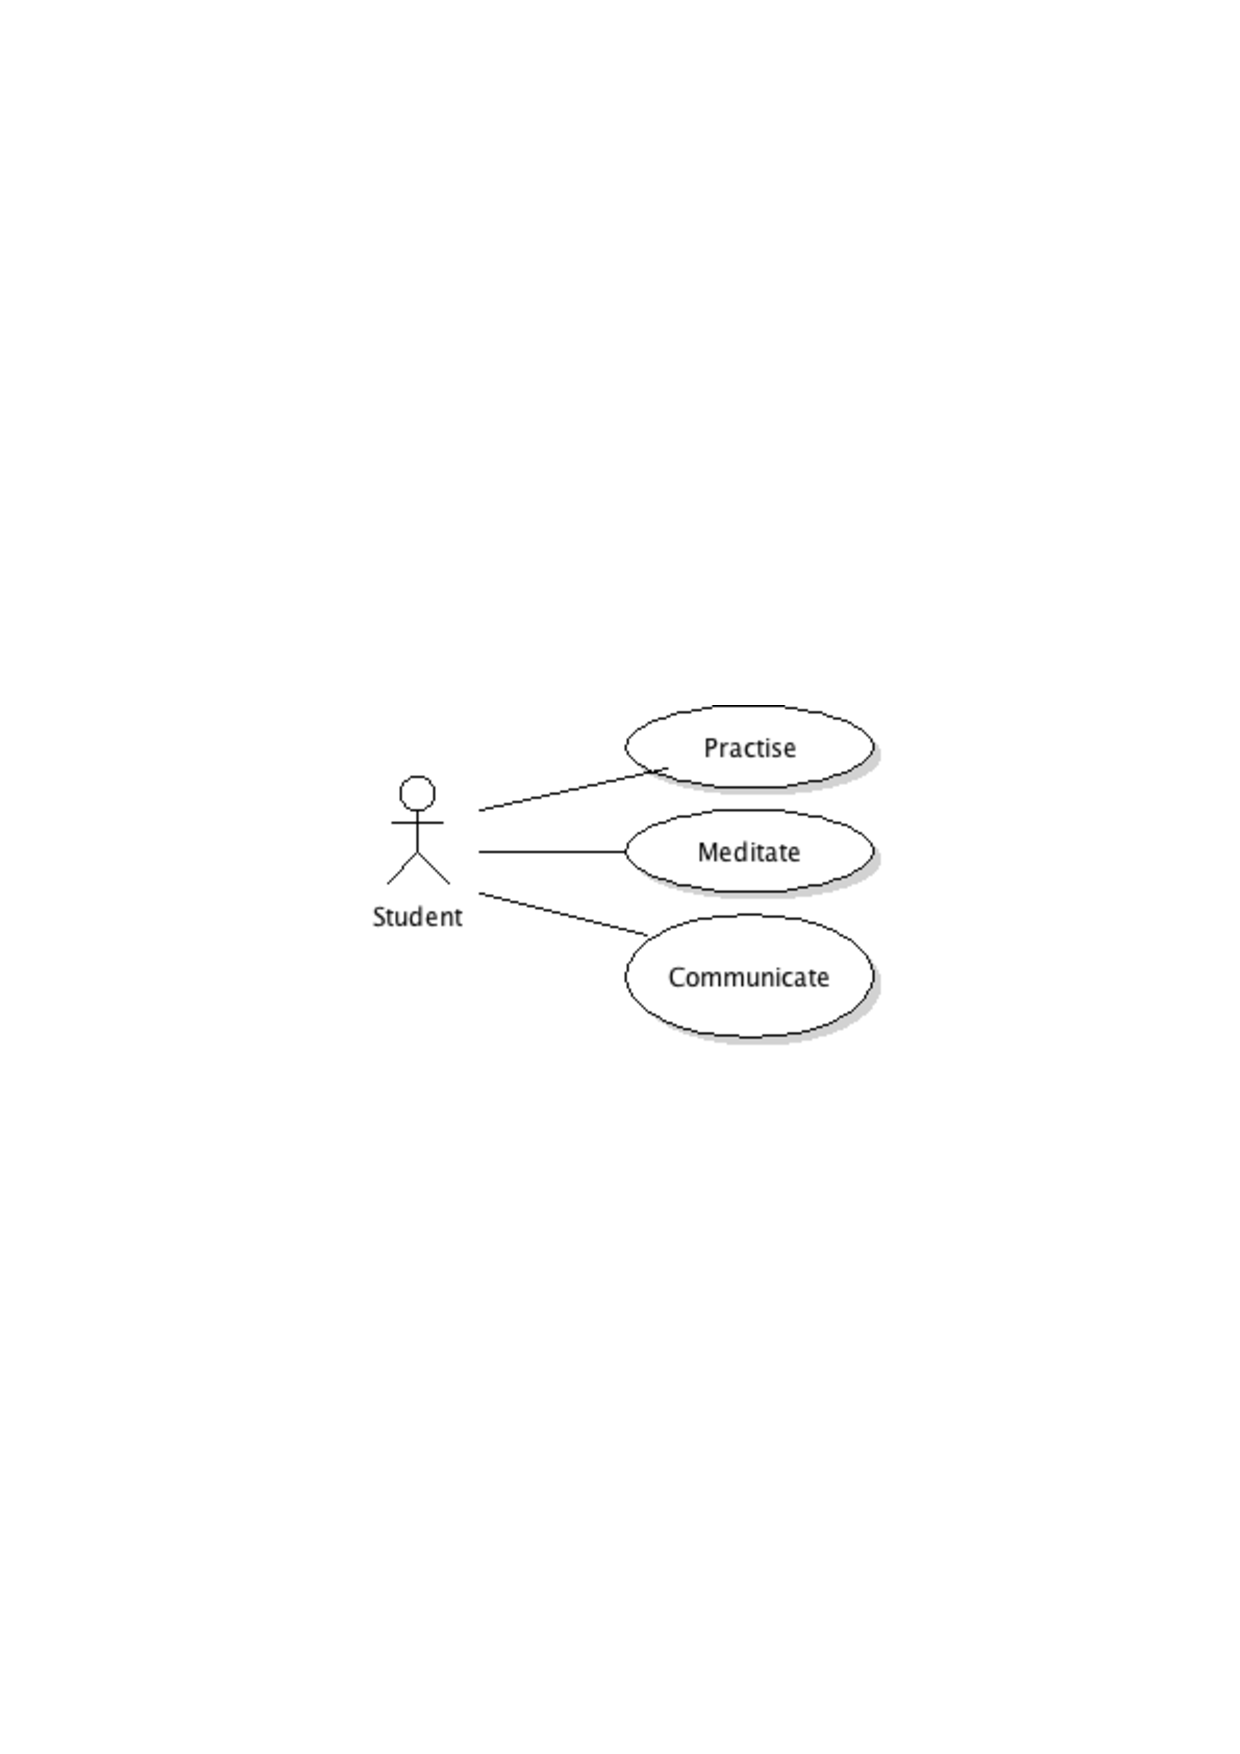
\includegraphics[width=\textwidth,  trim=2cm 12cm 2cm 12cm]{UML_figure/UC/student/UC_Student_General.pdf}
				\caption{Student Use Case : Overview}
			\end{center}
		\end{figure}
	\subsection{Practice}
		\begin{figure}[ht]
			\begin{center}
				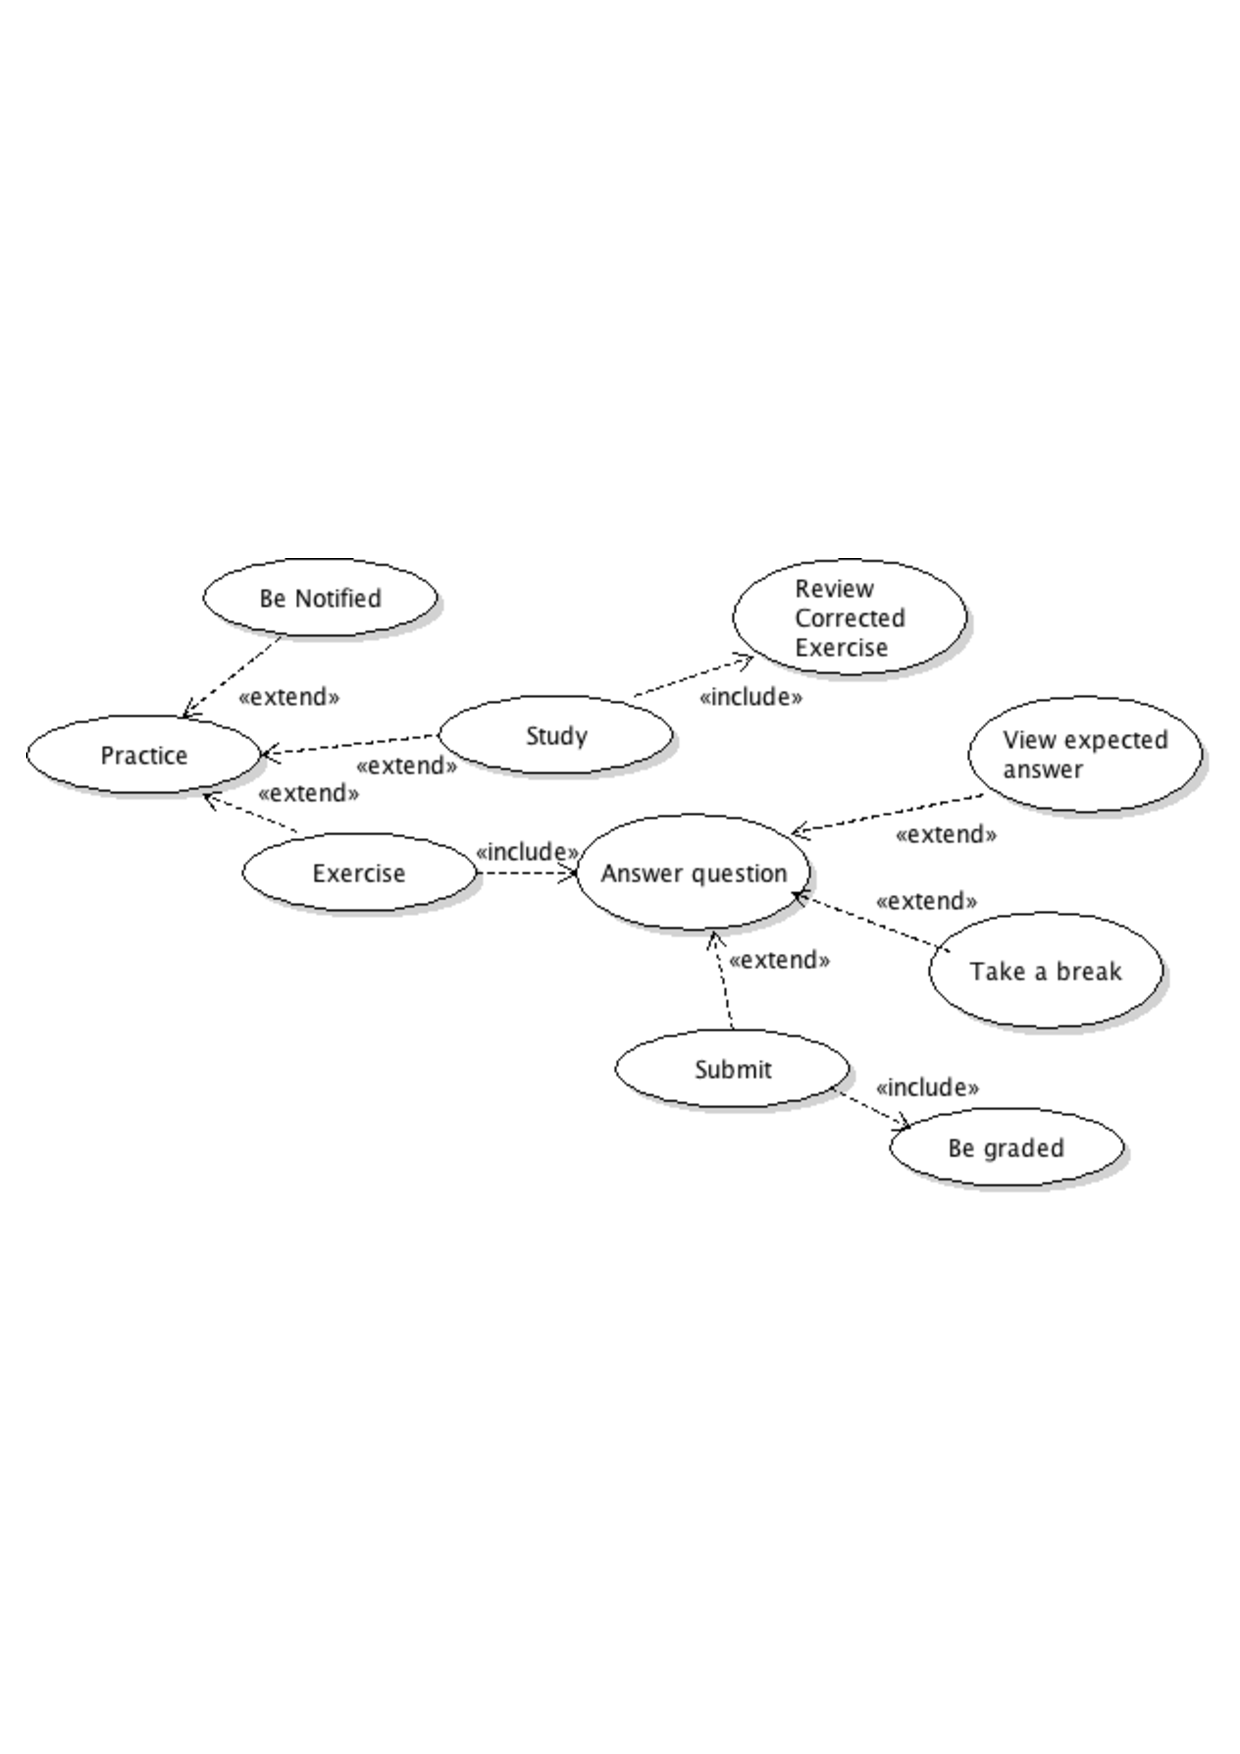
\includegraphics[width=\textwidth,  trim=2cm 10cm 2cm 10cm]{UML_figure/UC/student/UC_Student_Practice.pdf}
				\caption{Student Use Case : Practice}
			\end{center}
		\end{figure}
		\subsubsection{Be notified}
			The student is notified for new events.
		\subsubsection{Study}
			The student studies by reviewing corrected exercises.
		\subsubsection{Exercise}
			The student exercises by answering questions
		\subsubsection{Answer question}
			The student answers a set of question.
		\subsubsection{View expected answer}
			The student has optionally access to the corrected version.
		\subsubsection{Take a break}
			The student takes a break and resume the exercise later.
		\subsubsection{Submit}
			The student can submit his answer form.
		\subsubsection{Be graded}
			The student is also graded by the platform AFTER he submits his answer form.		
	\subsection{Meditate}
		\begin{figure}[ht]
			\begin{center}
				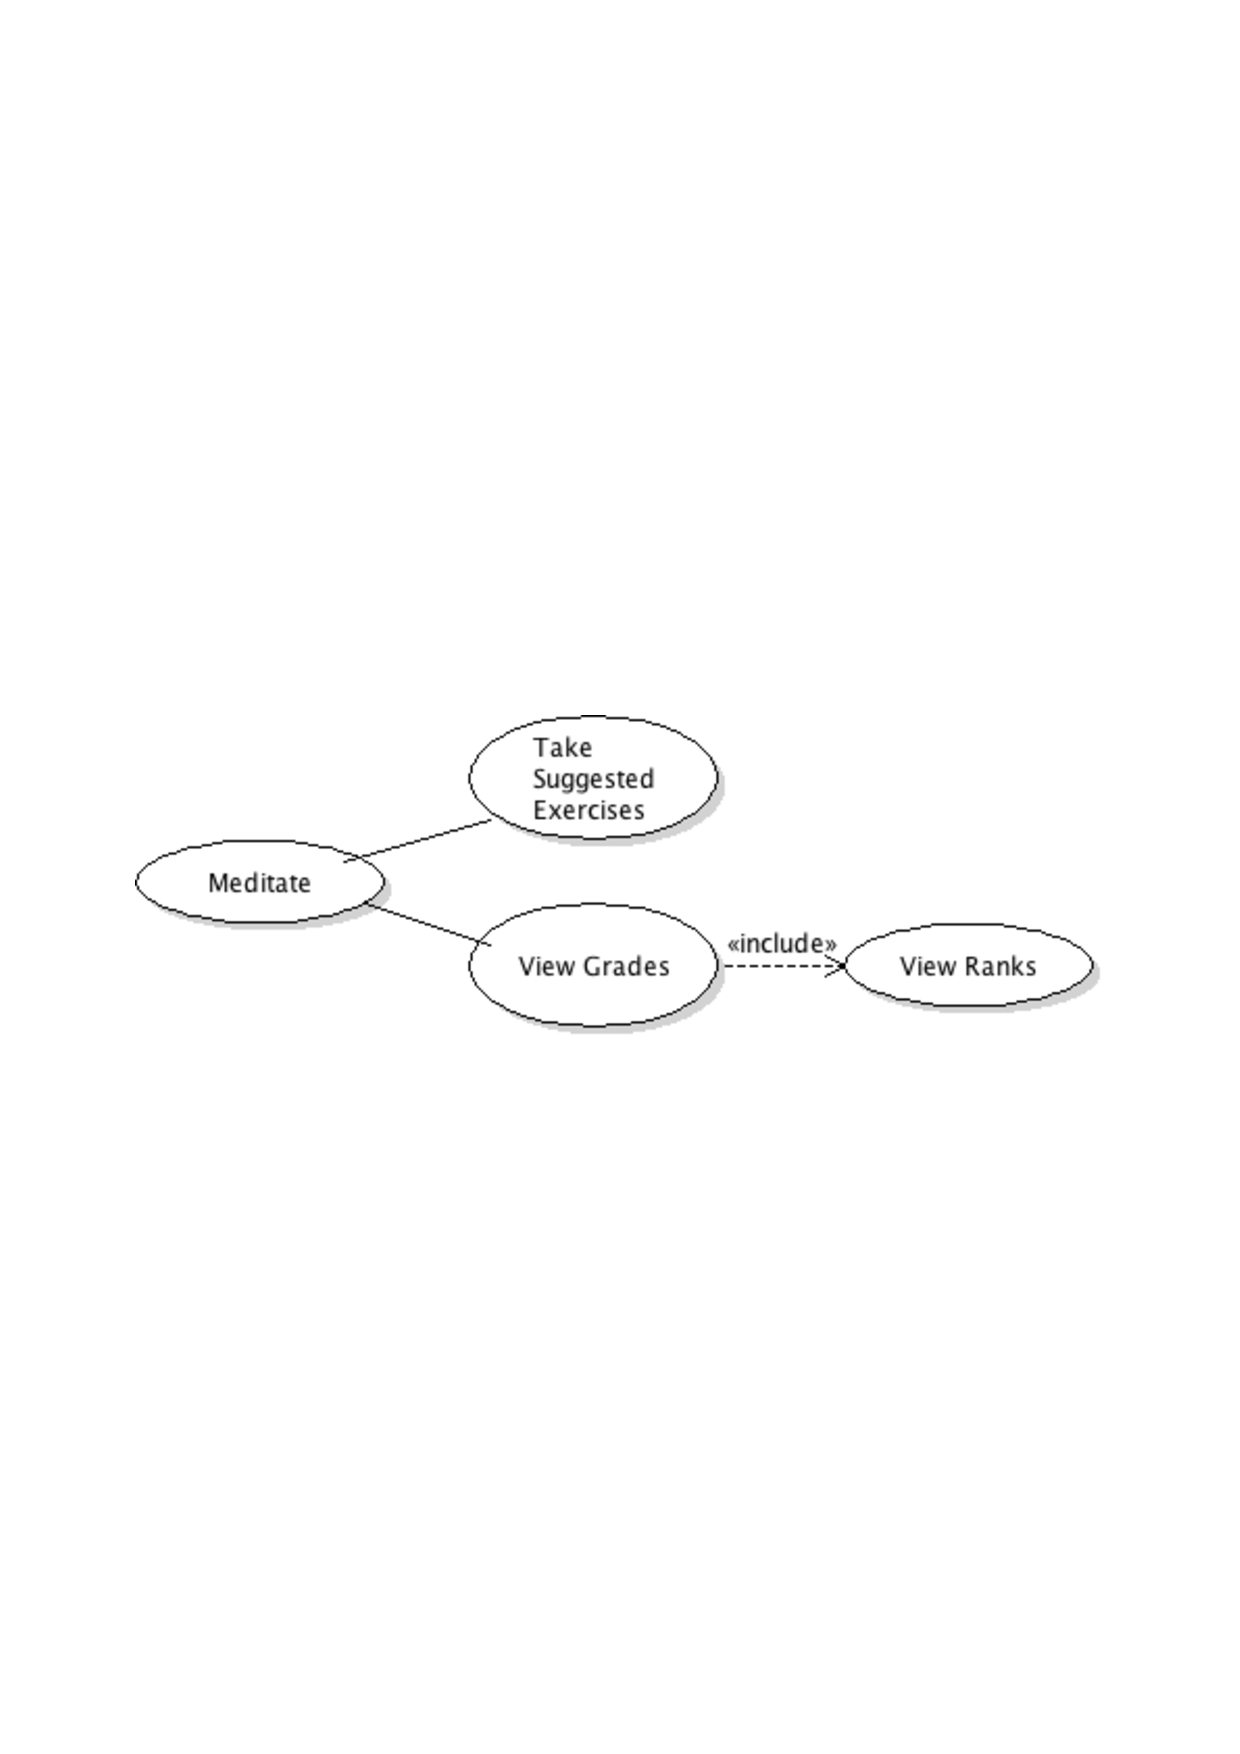
\includegraphics[width=\textwidth,  trim=2cm 12cm 2cm 12cm]{UML_figure/UC/student/UC_Student_Meditate.pdf}
				\caption{Student Use Case : Meditate}
			\end{center}
		\end{figure}
		\subsubsection{Take suggested exercises}
			The student access and starts a set of exercises according to their grade.
		\subsubsection{View Grades}
			The student can see their grade for each exercises.
		\subsubsection{View Ranks}
			The student can compare himself with other students.
%end student section
\newpage
%begin teacher section
\section{Teacher}
	\subsection{Overview}
		\begin{figure}[ht]
			\begin{center}
				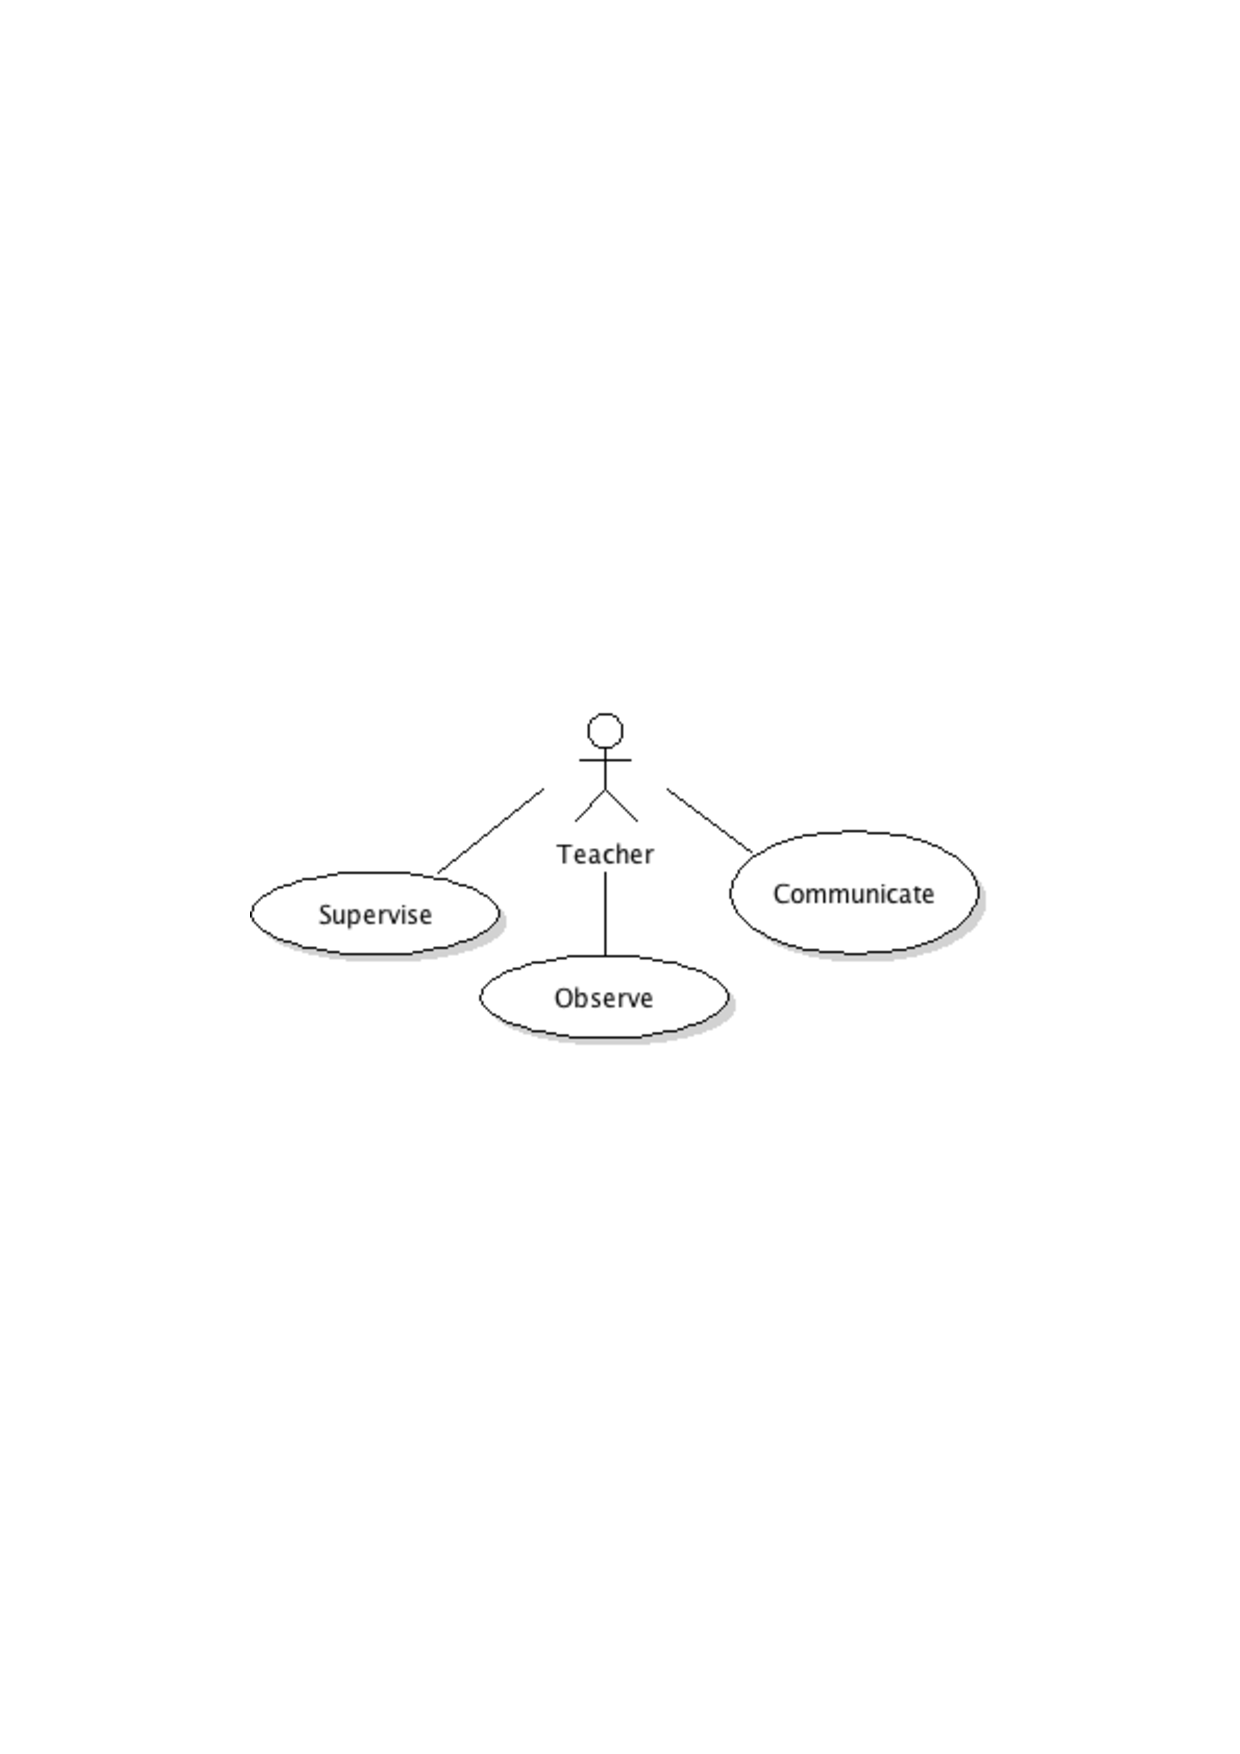
\includegraphics[width=\textwidth,  trim=2cm 11cm 2cm 12cm]{UML_figure/UC/teacher/UC_Teacher_General.pdf}
				\caption{Teacher Use Case : Overview}
			\end{center}
		\end{figure}
	\subsection{Supervise students}
		\begin{figure}[ht]
			\begin{center}
				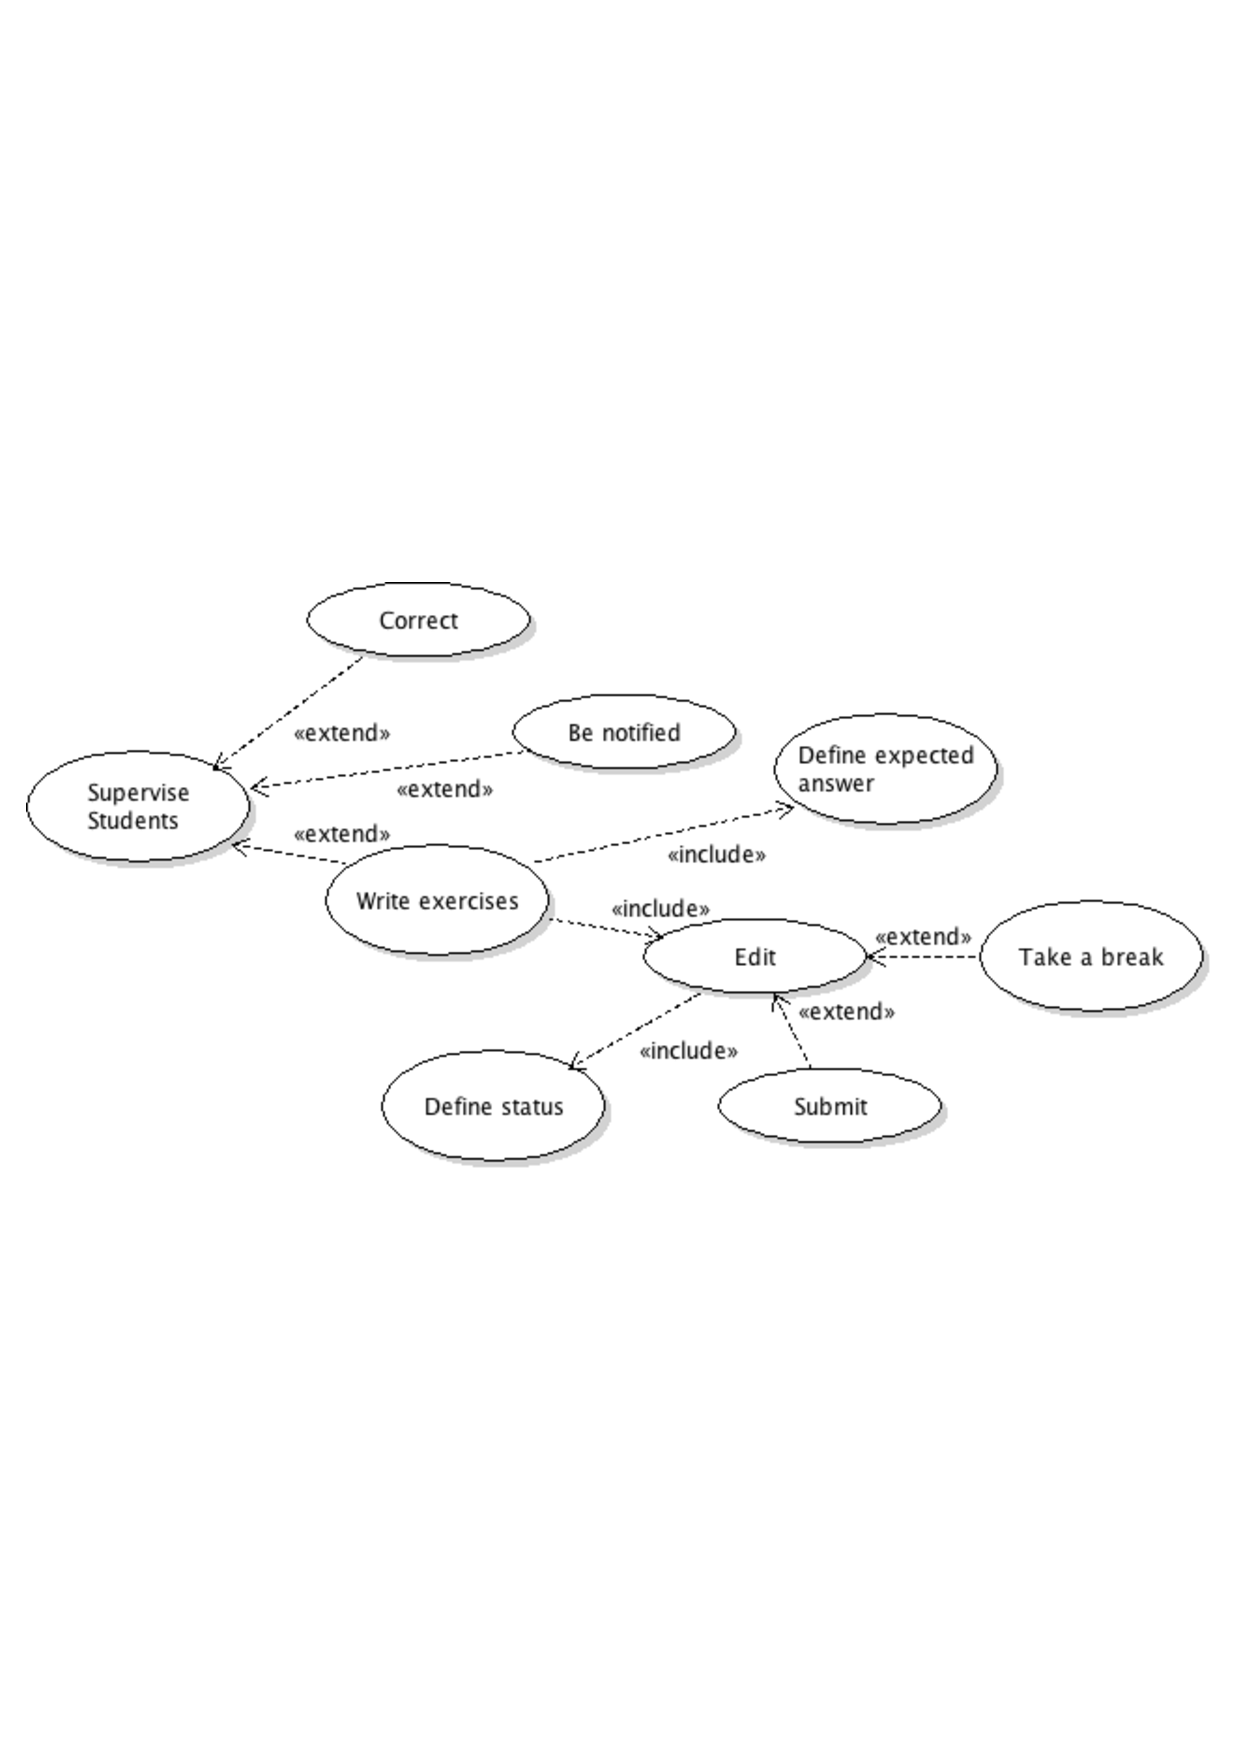
\includegraphics[width=\textwidth,  trim=2cm 10cm 2cm 10cm]{UML_figure/UC/teacher/UC_Teacher_Supervise.pdf}
				\caption{Teacher Use Case : Supervise students}
			\end{center}
		\end{figure}
		\subsubsection{Correct}
			The teacher has to grade students answers for questions which have no expected answers.
		\subsubsection{Be Notified}
			The teacher will be notified of events.
			For instance the teacher will be notified when one of his exercises is online.
		\subsubsection{Write exercises}
			The teacher supervises his students by writing exercises.
		\subsubsection{Define expected answer}
			When the teacher writes exercises, he can optionally define an expected answer.
		\subsubsection{Edit}
			The teacher can edit any exercise at anytime.
		\subsubsection{Define Status}
			The teacher attaches a status to an exercise.
		\subsubsection{Take a break}
			The teacher can resume his exercise later.
		\subsubsection{Submit}
			The teacher submits his exercise which can be viewed by student according to the exercise status defined by the teacher.
	\newpage
	\subsection{Observe}
		\begin{figure}[ht]
			\begin{center}
				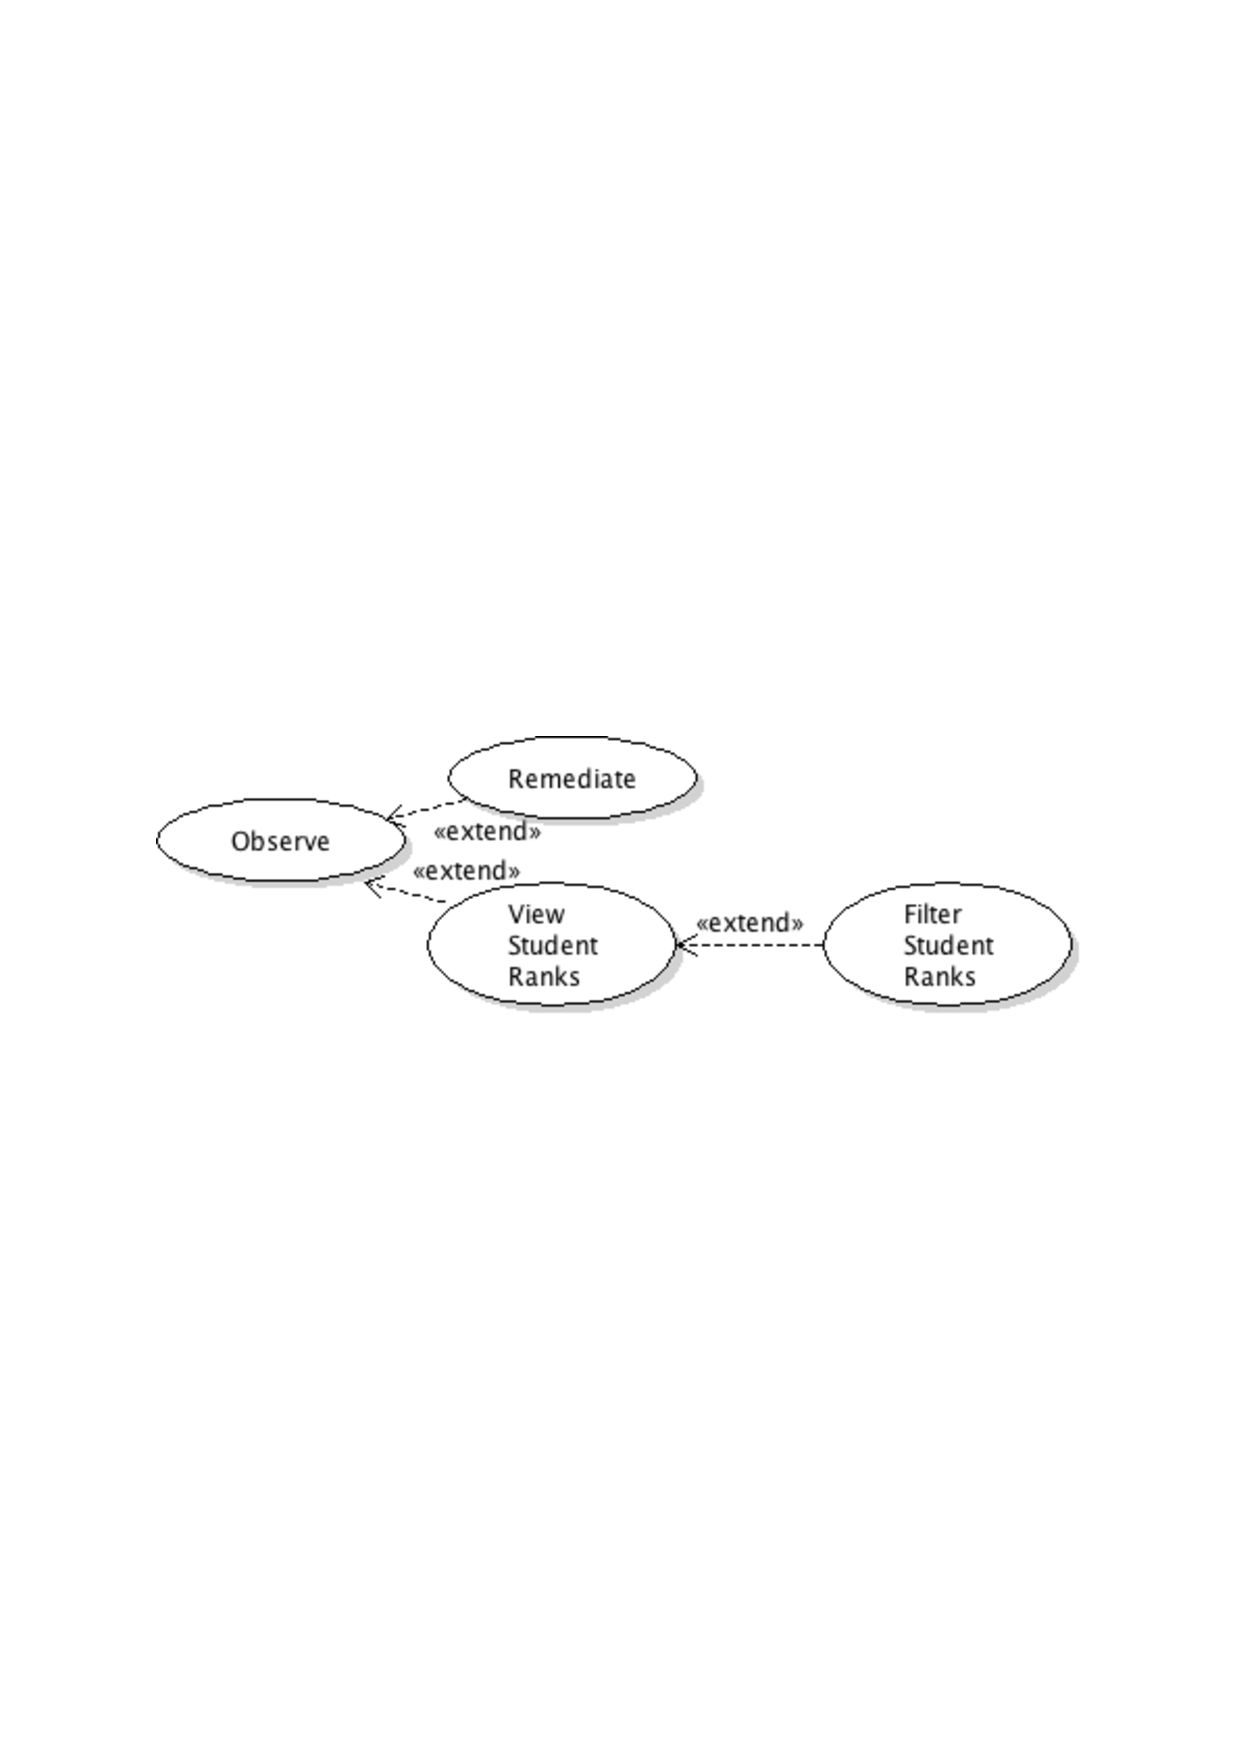
\includegraphics[width=\textwidth,  trim=2cm 12cm 2cm 12cm]{UML_figure/UC/teacher/UC_Teacher_Observe.pdf}
				\caption{Teacher Use Case : Observe}
			\end{center}
		\end{figure}
		\subsubsection{Rank}
			The teacher sees all the grades of students who took his exercises.
		\subsubsection{Filter}
			The teacher can filter the grades according to some parameters.
			The parameters can be the identifier of a group, the year for instance.
		\subsubsection{Remediate}
			The teacher can provide exercises for a group of students in trouble with some specific subject of the course according to their grades.
%end teacher section
\newpage
%begin administrator section
\section{Administrator}
	\subsection{Overview}
		\begin{figure}[ht]
			\begin{center}
				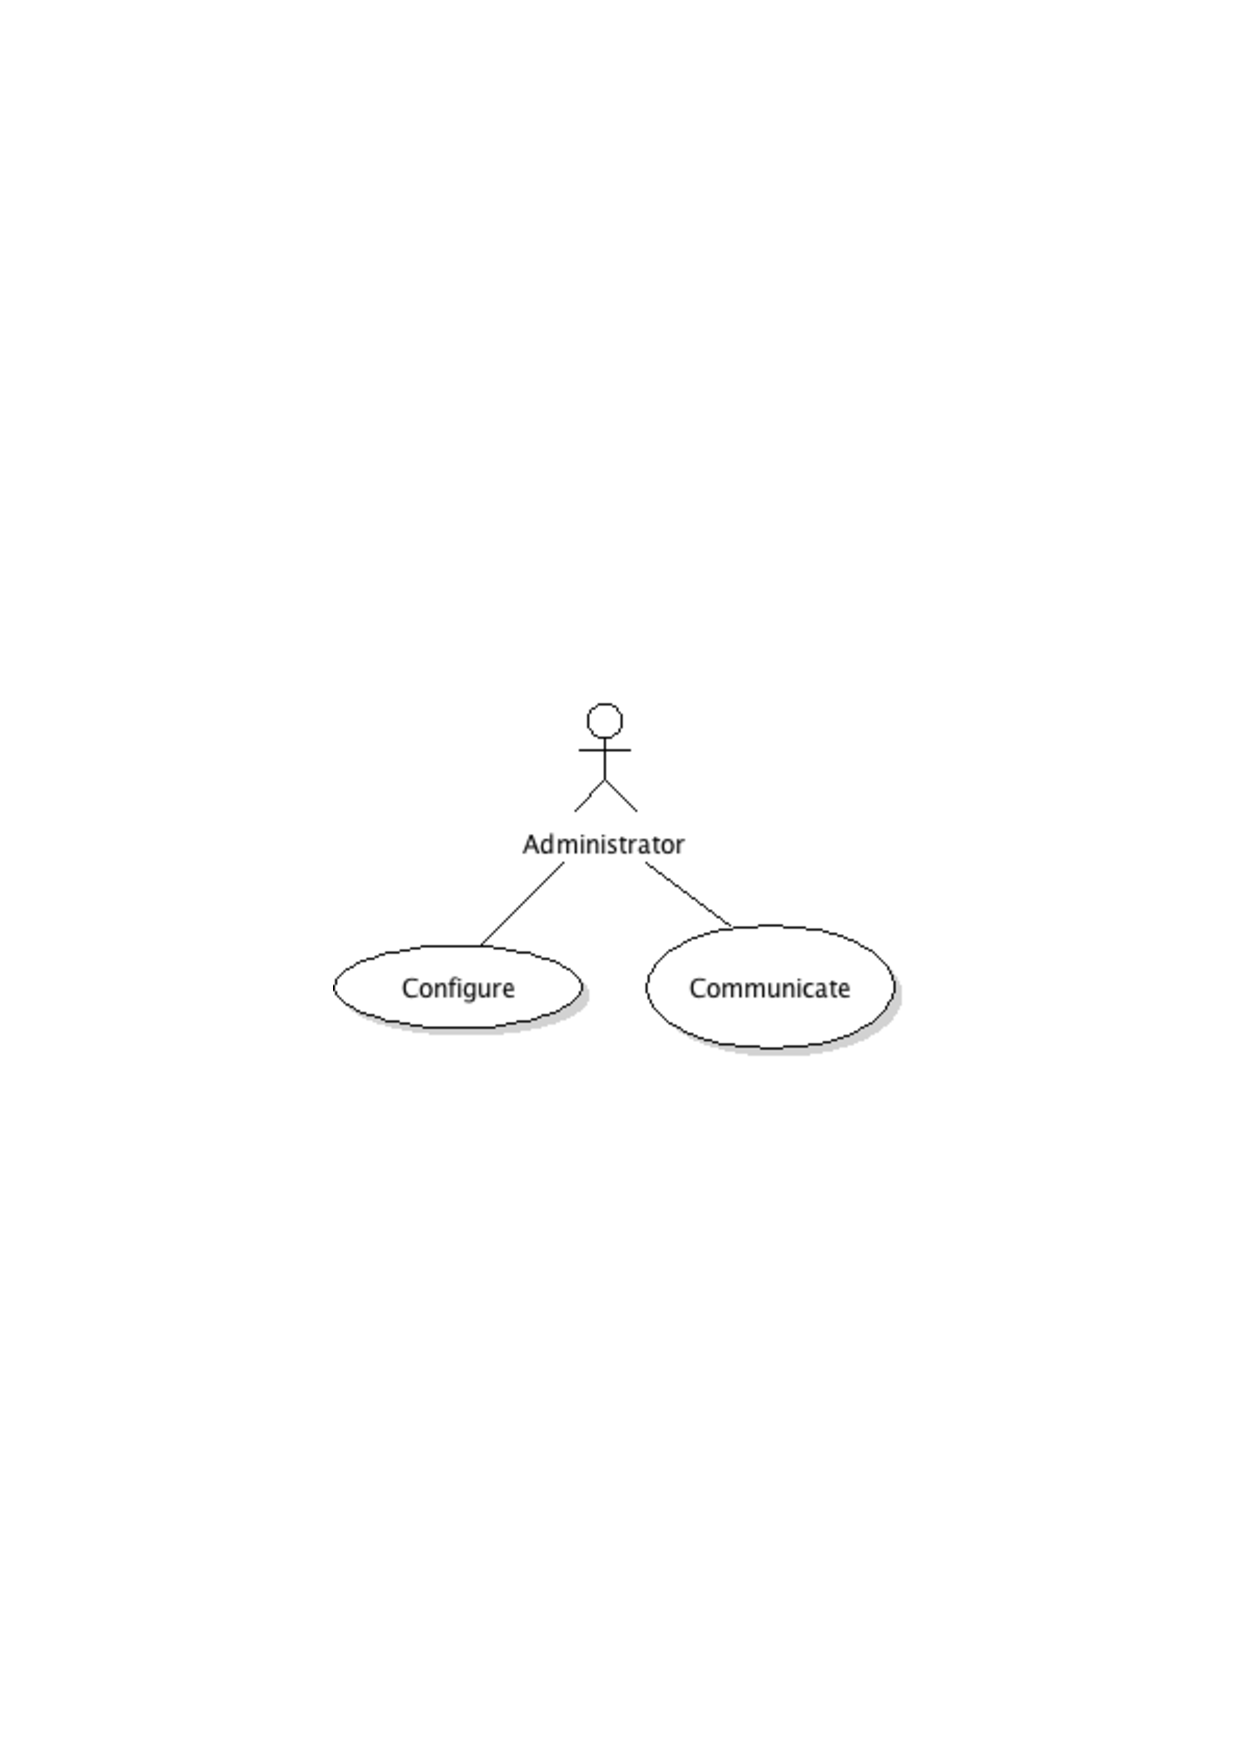
\includegraphics[width=\textwidth, trim=2cm 12cm 2cm 12cm]{UML_figure/UC/administrator/UC_Administrator_General.pdf}
				\caption{Administrator Use Case : Overview}
			\end{center}
		\end{figure}
	\subsection{Supervise the platform}
		\begin{figure}[ht]
			\begin{center}
				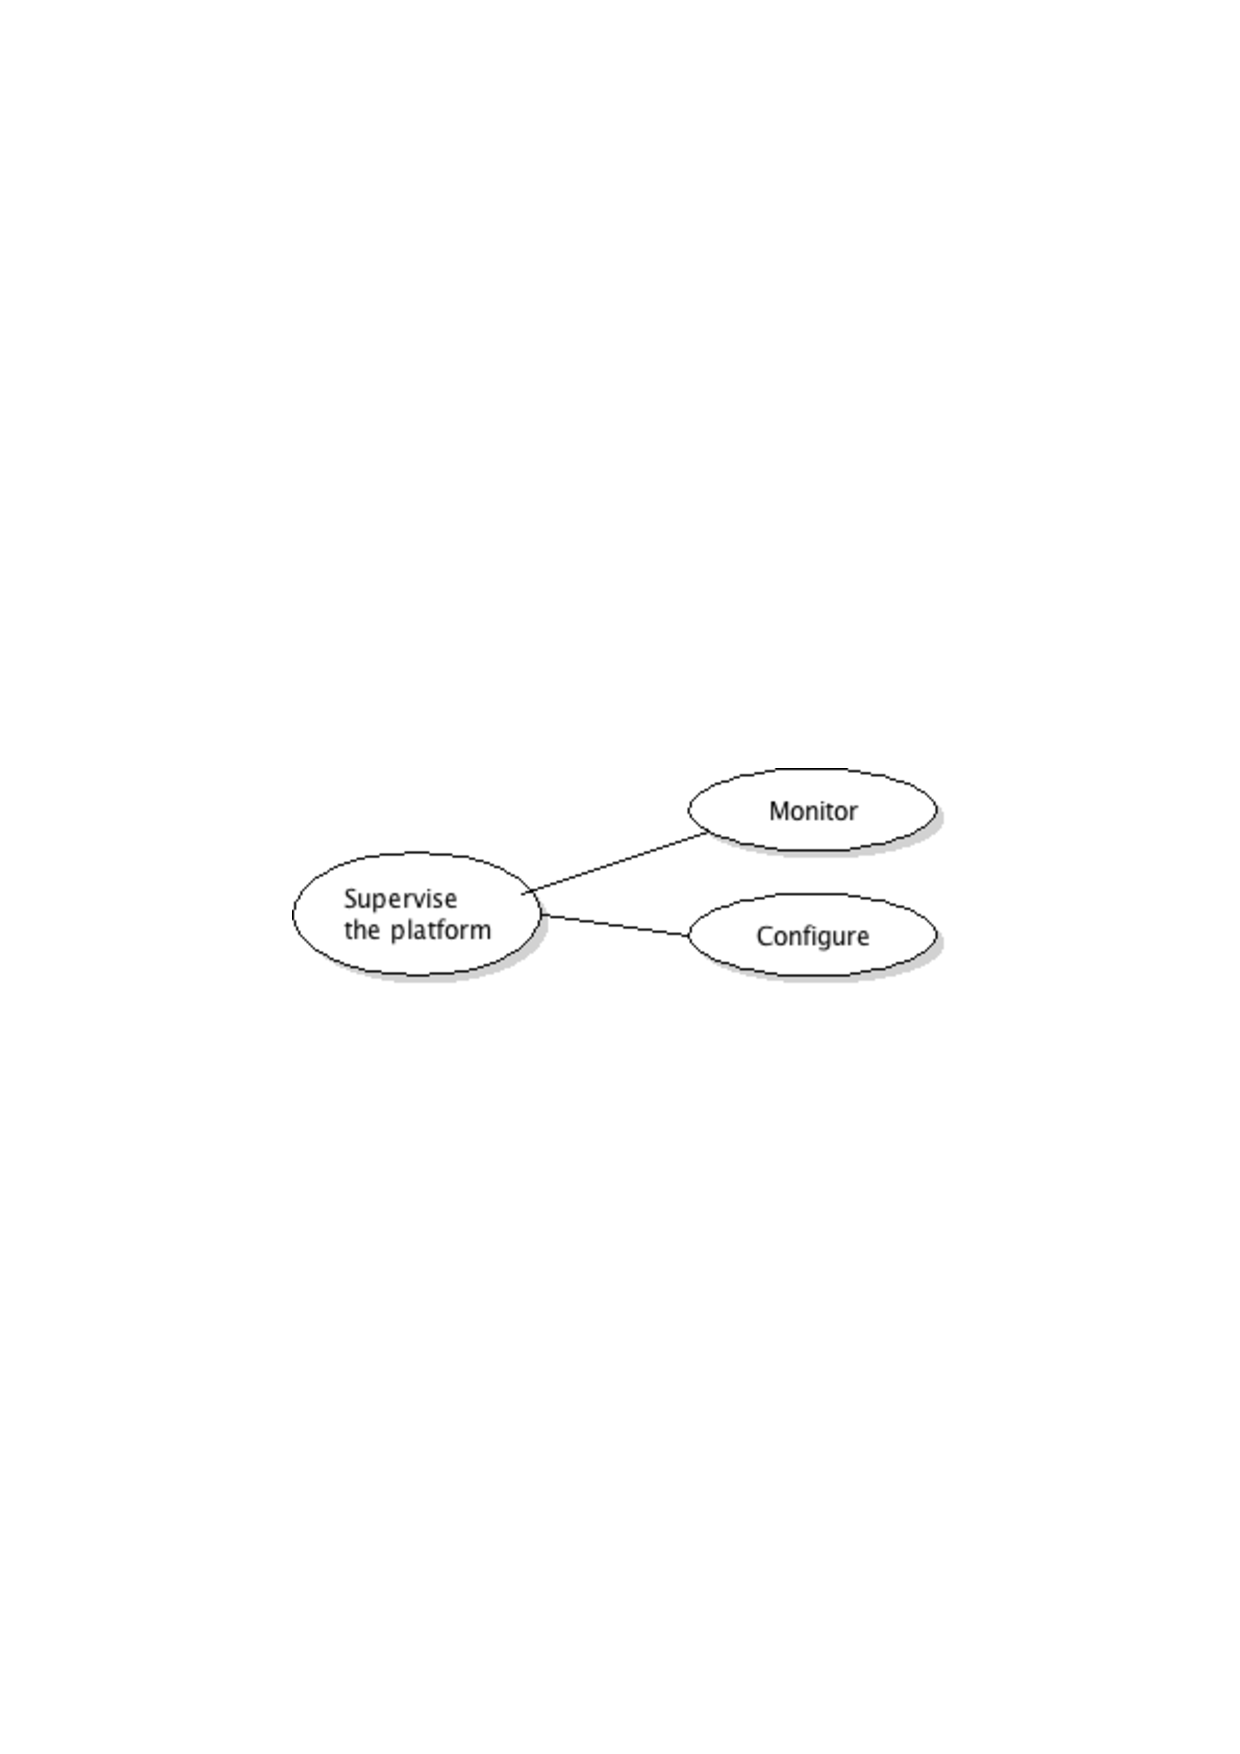
\includegraphics[width=\textwidth, trim=2cm 12cm 2cm 12cm]{UML_figure/UC/administrator/UC_Administrator_Supervise.pdf}
				\caption{Administrator Use Case : Supervise the platform}
			\end{center}
		\end{figure}
		\subsubsection{Be notified}
			The administrator will be notified by events such as critical issue.
		\subsubsection{Monitor}
			The administrator inspects the log.
		\subsubsection{Configure}
			The administrator configures the platform.
%end administrator section
\newpage
%begin common user section
\section{Common registered user}
	\begin{figure}[ht]
		\begin{center}
			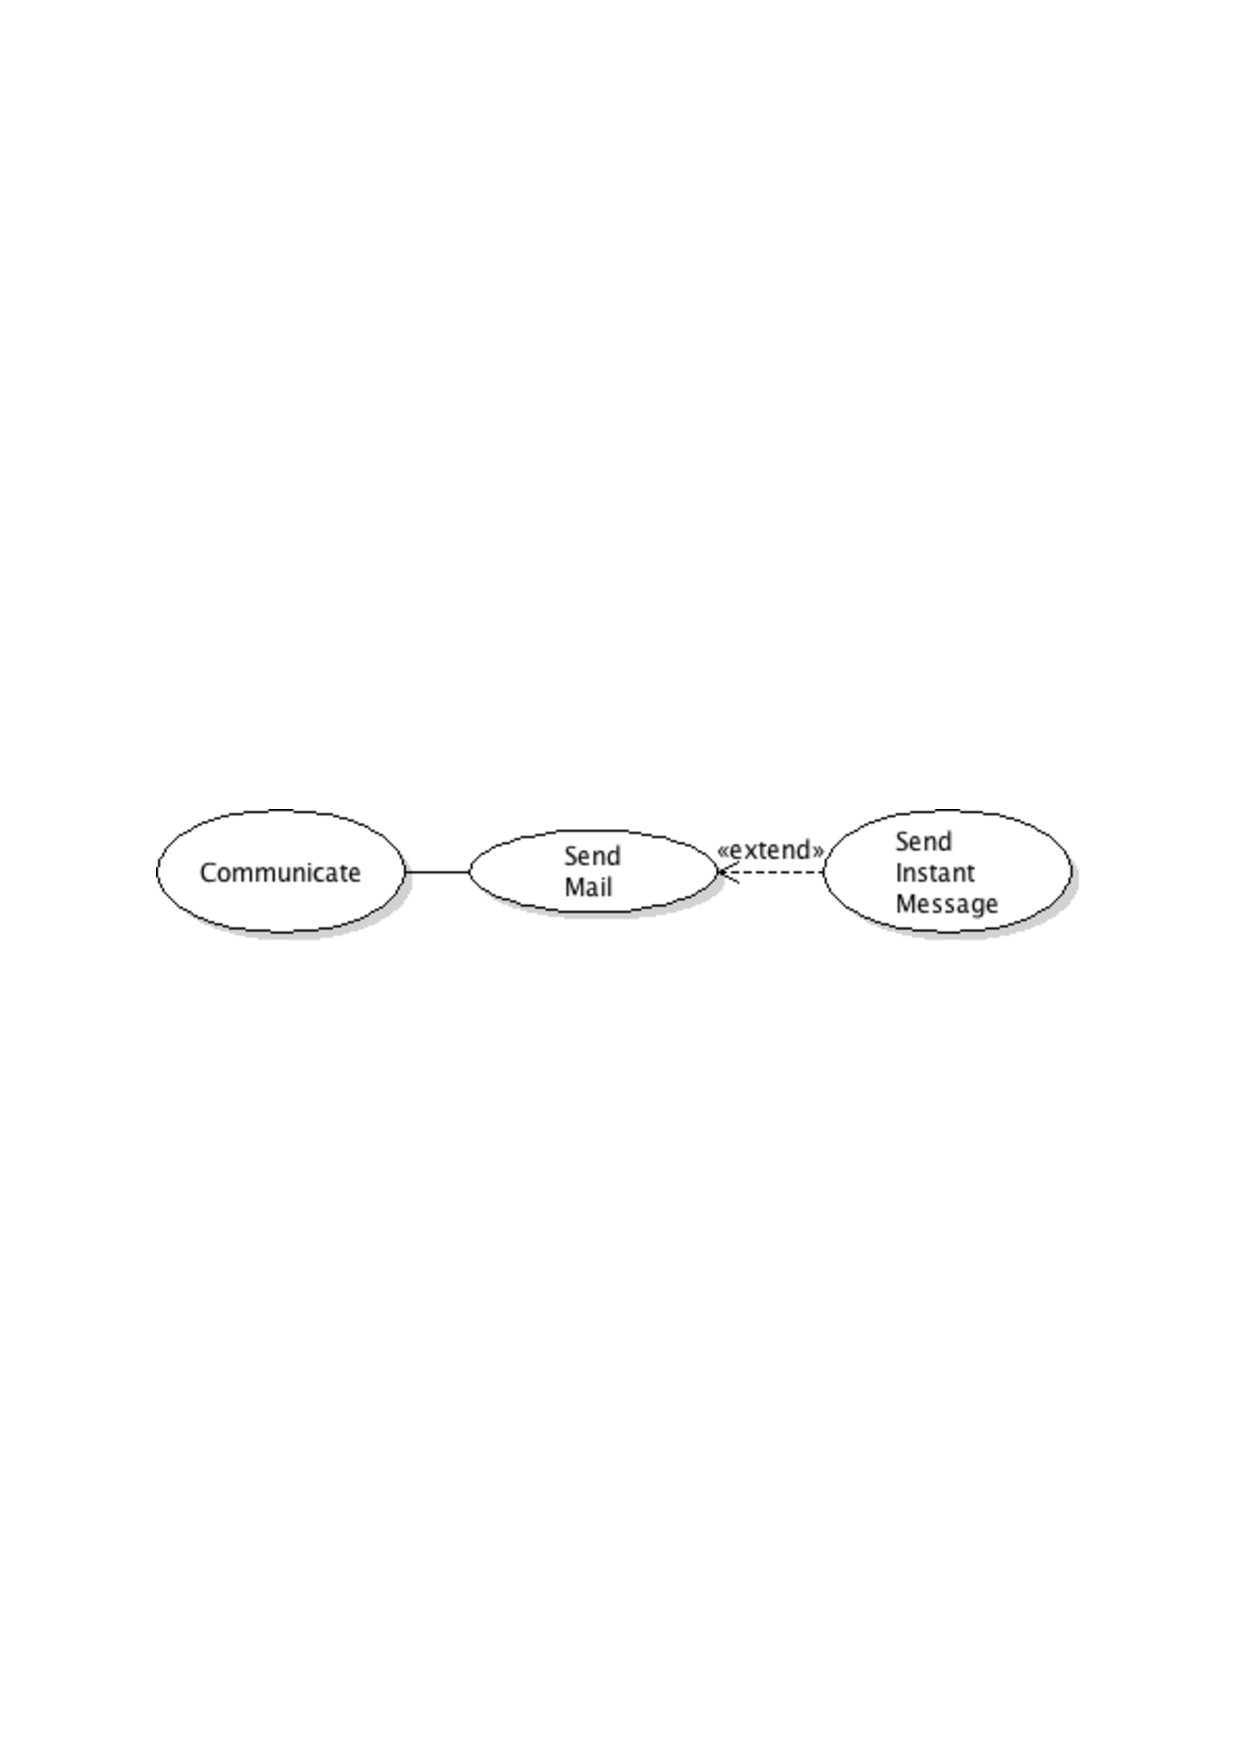
\includegraphics[width=\textwidth,  trim=2cm 12cm 2cm 12cm]{UML_figure/UC/common/UC_Common_Communicate.pdf}
			\caption{Registered user Use Case : Communicate}
		\end{center}
	\end{figure}
	\subsection{Communicate}
		\subsubsection{Send Mail}
			Identifed user communicate by mail exchange.
		\subsubsection{Send Instant Message}
			Identifed user communicate by instant message exchange.
%end common user section













